\chapter{Problem Definition}

Tools such as vector analyzers are heavy and expensive, costing tens of
thousands of dollars.  There is need of a tool for students and teachers to
help teach electronics and similar courses.  Currently, there are no feasibly
affordable tools to show the frequency response and phase of a circuit,
amplifier, or control loop, and the learning experience is hindered by this
gap.

\section{Problem Scope}

This project will produce a portable frequency response analyzer.  It will
communicate data with a computer through USB in order to form a Bode plot of
the frequency and phase response of the circuit.

\section{Technical Review}

Proper circuit analysis is a fundamental practice in the field of engineering,
since it is necessary for every electronic device on the market.  As a result,
it is the goal of every engineering institution to give students a strong basis
in circuit design and analysis.

Currently, this is done mainly through lecture and labs.  A professor stands in
front of a classroom and delivers a lecture based on PowerPoint slides that
they have created.  It is expected that, from this, students grasp the concepts
necessary to make them proficient in working with electronics.  Although this
may be a seemingly efficient way to broadcast the fundamentals to many people,
it must be augmented with practice.

Then, there is the lab section of the class.  Students are asked to put
together a circuit and then observe it using a measuring device. Unfortunately,
few such devices are available for frequency-domain work.

It is the goal of this project to help remedy this situation.  This USB
Gain/Phase Analyzer is a cheap, portable tool.  With this, a teacher would have
the ability to bring circuits to class and actually demonstrate fundamentals to
their students.  This would inevitably enhance the effectiveness of their
lectures because students would see how these circuits respond in application.
The aim, here, is to help a teacher captivate his/her students.

Additionally, the analyzer is a tool that students can afford.  In a lab, they
could now be asked to design something, increasing the creative thinking of the
prospective engineer.  With this tool, they can now do more meaningful analysis
and see their devices' behaviors on real world signals.  Also, the device is
portable enough that students could take it home and do lab work there, without
needing to spend thousands of dollars on lab equipment.

\section{Design Requirements}

\subsection{Context-Level Constraints}

This project is producing one gain/phase analyzer system. As shown in \autoref{fig:contextdiag},
 the device connects to a PC for user control and viewing of data. It has one
Drive output, with which it applies a stimulus to a Device Under Test (DUT),
and two Sense inputs, with which it detects the amplitude and phase of signals
before and after the DUT. The device will also have an Adapter port, with which
it can connect to external adapters for measuring various types of DUTs.  The
gain/phase analyzer system, in addition to the hardware, comprises PC Software
with which the end user may start analyses and view results.

\begin{figure}[H]
\centering
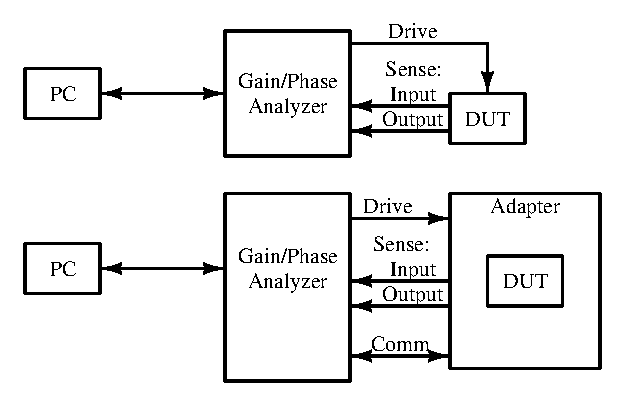
\includegraphics{contextdiagram}
\caption{Gain/Phase Analyzer Context Diagram}
\label{fig:contextdiag}
\end{figure}

\subsection{System-Level Constraints}

As shown in \autoref{fig:systemdiag}, the analyzer uses a \emph{Synthesizer} to
generate the stimulus signal, and an \emph{Output Amplifier} to provide the stimulus
signal to the DUT, at up to 1.25 V RMS and up to 150 MHz. \emph{Input Filters}, an
\emph{Input Switching Network} and the \emph{Input Detector} provide a signal corresponding
to the amplitude of the signals at the Sense ports. The Input Switching Network
can also select a \emph{Phase Reference} to be summed with the signals for phase
measurement. These are digitized by an \emph{Analog-Digital Converter} to be processed
by the \emph{Microprocessor}. The Microprocessor then interfaces with the \emph{Software} via
the \emph{PC Interface}.

\begin{figure}[H]
\centering
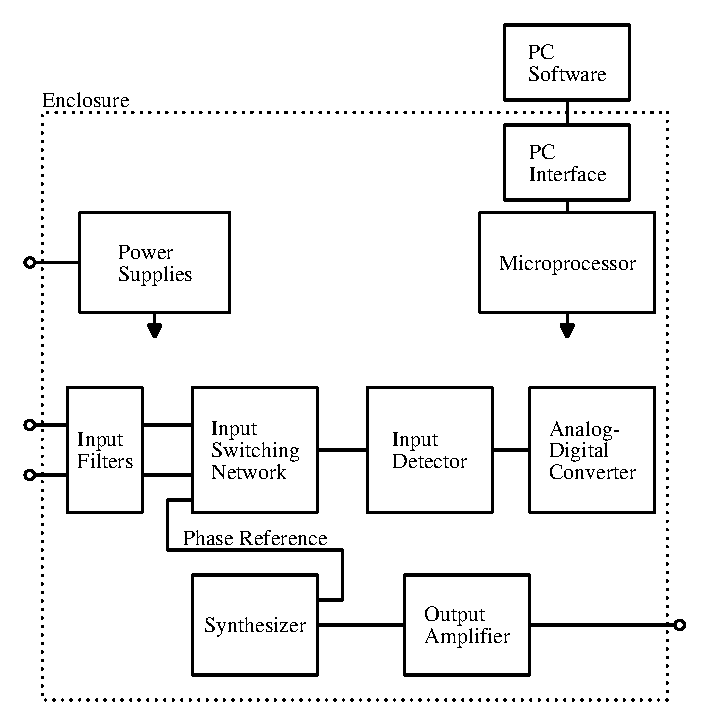
\includegraphics{systemdiagram}
\caption{Gain/Phase Analyzer System Diagram}
\label{fig:systemdiag}
\end{figure}
